\documentclass[10pt]{article}

\usepackage[utf8]{inputenc}
\usepackage[T1]{fontenc}
\usepackage{amsmath,amssymb,amsthm}
\usepackage{algorithm}
\usepackage{algpseudocode}
\usepackage{hyperref}
\usepackage{cleveref}
\usepackage{booktabs}
\usepackage{tikz}
\usepackage{geometry}
\geometry{margin=1in}

\newtheorem{theorem}{Theorem}
\newtheorem{lemma}{Lemma}

% Fix duplicate hyperref anchors produced by algorithmicx line numbers.
% See e.g. the common "ALG@line" duplicate destination issue.
\makeatletter
\providecommand{\theHalgorithm}{\arabic{algorithm}}
\providecommand{\theHALG@line}{}
\renewcommand{\theHALG@line}{\theHalgorithm.\arabic{ALG@line}}
\makeatother

\title{A very simple \(O(n + k\log k)\) polygon triangulation (brainstorm draft)}
\author{Pavel Shpagin \and Vasyl Tereschenko}
\date{\today}

\begin{document}
\maketitle

\begin{abstract}
This is a \emph{brainstorming} draft for a drastically simplified presentation of an instance-sensitive triangulation algorithm.
The target bound is \(O(n + k\log k)\), where \(k\) is the number of local maxima (equivalently local minima) with respect to the \(y\)-direction.
Under general position, \(1 \le k \le \lfloor n/2 \rfloor\); for convex polygons, \(k=1\).
The key idea (inspired by \texttt{original\_paper.txt}) is to process only reflex extrema in sorted \(y\)-order, create a sparse set of ``horizontal-chord'' connections that eliminate all split/merge vertices, obtain \(y\)-monotone pieces, and then triangulate those in linear time.

\medskip
\noindent\textbf{Status:} not a finished algorithm description; contains open issues and alternative implementation paths.
\end{abstract}

\section{Goal and scope}
We want an algorithm that is:
\begin{itemize}
  \item \textbf{Conceptually minimal}: few cases, few data structures, easy to implement.
  \item \textbf{Instance-sensitive}: \(O(n + k\log k)\) rather than \(O(n\log n)\) in the typical case.
  \item \textbf{Competitive in practice}: dominated by a small number of balanced-tree operations plus cache-friendly pointer walks.
\end{itemize}

We focus on simple polygons without holes and assume general position (no horizontal edges / equal \(y\)).

\section{Definitions (minimal)}
Let \(P=(v_0,\dots,v_{n-1})\) be a simple polygon in CCW order.
Classify vertices by comparing neighbor \(y\)-coordinates:
\begin{itemize}
  \item \textbf{local maximum}: \(y(v_{i-1}) < y(v_i)\) and \(y(v_{i+1}) < y(v_i)\)
  \item \textbf{local minimum}: \(y(v_{i-1}) > y(v_i)\) and \(y(v_{i+1}) > y(v_i)\)
  \item \textbf{split}: reflex local maximum
  \item \textbf{merge}: reflex local minimum
\end{itemize}
Let \(k\) be the number of local maxima (equivalently local minima).
We also use \(k_r\) for the number of \emph{reflex extrema} (split+merge vertices).
For simple polygons in general position, \(k_r \le k-1\), hence \(k_r \le \lfloor n/2 \rfloor - 1\); for convex polygons \(k_r=0\).

\paragraph{Horizontal chord (concept).}
Given a vertex \(v\) at height \(y(v)\), the \emph{horizontal chord} at \(v\) is the pair of intersections of the horizontal line \(y=y(v)\) with the polygon boundary to the left and right of \(v\).
Operationally, this is a (two-sided) horizontal ray-shooting query on \(\partial P\).

\section{High-level algorithm sketch}
\subsection{Phase A: one sort}
\begin{enumerate}
  \item Traverse \(\partial P\) once, identify all split/merge vertices, and store them in an array \(R\).
  \item Sort \(R\) by \(y\)-coordinate (bottom-to-top or top-to-bottom). Cost: \(O(k\log k)\).
\end{enumerate}

\subsection{Phase B: eliminate reflex extrema by ``chords''}
Process reflex extrema in sorted order.
For each reflex extremum \(r\):
\begin{itemize}
  \item Find the two boundary edges \(e_L\) and \(e_R\) intersected by the horizontal line through \(r\) on the left and right of \(r\).
  \item Choose a diagonal endpoint according to a small rule set that mirrors the classical monotone-decomposition sweep:
    \begin{itemize}
      \item At a \textbf{split} vertex, connect upward to the current ``helper'' on the chain immediately left.
      \item At a \textbf{merge} vertex, connect downward if needed and update the helper state of the chain immediately left.
    \end{itemize}
\end{itemize}

\paragraph{Two implementation paths.}
The above can be implemented in two ways:
\begin{itemize}
  \item \textbf{(B1) Classical sweep}: maintain a balanced BST of active edges and do predecessor queries at event heights (this is basically Garey/de~Berg, but we only \emph{emit} diagonals at split/merge and try to avoid per-regular-vertex work via laziness).
  \item \textbf{(B2) Reflex-chord pointer-walk}: maintain a linked polygon representation and, when processing the next reflex extremum in \(y\)-order, walk two pointers along the boundary until they hit the chord support edges; splice out the processed region and update local reflex bookkeeping. The hope is that the total pointer movement is \(O(n)\) (each boundary edge is ``advanced past'' only a constant number of times).
\end{itemize}

\paragraph{Why this might be simpler.}
In the best case, Phase B reduces to:
\begin{itemize}
  \item a single global sort of \(k\) reflex extrema,
  \item plus a linear amount of boundary pointer advancement,
  \item plus \(O(k)\) small local updates / splices.
\end{itemize}

\subsection{Phase C: triangulate monotone pieces}
Once all split/merge vertices are eliminated by diagonals, the polygon is partitioned into \(y\)-monotone pieces.
Each piece is triangulated in linear time via the standard stack algorithm.
Total over all pieces is \(O(n)\).

\section{Complexity target}
\begin{itemize}
  \item Sort reflex extrema: \(O(k_r\log k_r) \subseteq O(k\log k)\).
  \item Pointer advancement / local splicing over the whole run: \(O(n)\) (goal; must be proved carefully).
  \item Optional balanced-tree operations if we keep a BST for ordering: \(O(k\log k)\).
\end{itemize}

\section{Open issues / questions}
\begin{itemize}
  \item \textbf{Correctness}: can the chord-based rules be stated so that they are \emph{provably equivalent} to the classical sweep (and thus guaranteed non-crossing + monotone partition)?
  \item \textbf{``Without events''?} Even if we only sort split/merge vertices, convex extrema can still affect which chain is immediately left at a split/merge height. If we drop convex extrema entirely, we need an alternative argument/data structure to recover the same predecessor relation.
  \item \textbf{Robustness}: horizontal chord endpoints are generally interior points on edges, not vertices; a clean implementation must either (i) support edge splitting in a DCEL, or (ii) avoid materializing chord endpoints by using chain pointers (preferred).
  \item \textbf{Parameter choice}: should the paper parameter be \(k\)=\#(all extrema) or \(k_r\)=\#(reflex extrema)? The reflex-extrema parameter can be much smaller in practice and matches the chord intuition.
\end{itemize}

\section{Brainstorm: can we eliminate the BST entirely?}
The chain-sweep formulation from the CGAT paper uses a balanced BST to answer predecessor queries
(``which active chain is immediately left of the current event vertex?'').
Here we brainstorm directions to remove that BST while keeping a \(k\log k\)-type bound.

\subsection{Key observation: no swaps in the left-to-right order}
Active boundary chains (or edges) do not intersect each other.
If we view each active chain as a continuous \(x(y)\) function over the \(y\)-range where it is active, then two chains can swap left-to-right order only if they intersect at some height.
So the left-to-right order of simultaneously active chains is \emph{fixed} over any interval of \(y\) where the active set does not change.

\paragraph{What the BST is really doing.}
The BST is not needed because the order changes (it does not); it is needed because we must \emph{locate} the predecessor of a query \(x\)-coordinate among currently active chains.
So to remove the BST we need to avoid general predecessor search.

\subsection{Direction A: avoid predecessor search by ``horizontal chord'' pointer-walking}
This is the direction suggested by \texttt{original\_paper.txt}.
Informally:
\begin{itemize}
  \item Sort only a small set of special vertices (e.g., reflex extrema \(k_r\) or all extrema \(k\)) by \(y\).
  \item Process them bottom-to-top (or top-to-bottom).
  \item Maintain a linked representation of the current polygon boundary.
  \item For the current extremum \(v\), find the two boundary edges hit by the horizontal line \(y=y(v)\) by walking boundary pointers outward until they cross that height.
  \item Splice out the processed region and continue; charge all pointer movement to boundary edges so the total is \(O(n)\).
\end{itemize}

\paragraph{Why this could eliminate the BST.}
If the ``find chord supports'' step can be done by local pointer walks (rather than searching among all active edges),
then the only \( \log \) factor left is the initial sort of \(k\) (or \(k_r\)) events.

\paragraph{Hard parts (need real proofs).}
\begin{itemize}
  \item \textbf{Do new extrema appear?} After splicing and/or introducing chord-intersection vertices, new local extrema could appear. If so, we need a way to (i) detect them locally and (ii) insert them into the processing order without a global priority queue.
  \item \textbf{Correctness (non-crossing diagonals).} The chord endpoints are typically interior points on edges. We need a clean way to turn chords into vertex-to-vertex diagonals (or avoid materializing new vertices by using chain pointers).
  \item \textbf{Equivalence to textbook sweep.} The cleanest route to correctness might still be an equivalence argument: show that each splice corresponds to the same diagonal the classical monotone-decomposition sweep would insert.
\end{itemize}

\subsubsection{Direction A.1: make it concrete (data + invariants)}
The goal is to replace ``predecessor in a global ordered set of active edges'' by
\emph{component-local pointer walks} on the polygon boundary.

\paragraph{Representation.}
Maintain each current polygon component as a cyclic doubly-linked list of its boundary vertices.
Each original vertex stores:
\begin{itemize}
  \item its neighbor pointers in the current component,
  \item its original coordinates,
  \item whether it is a reflex extremum (split/merge) in the \emph{current} component (this can change after cutting),
  \item a pointer to its node in the component's reflex list (if present).
\end{itemize}

\paragraph{Reflex list (component-local).}
For each component, maintain a doubly-linked list of \emph{active reflex extrema} in that component ordered along the boundary.
Additionally, we maintain a constant amount of ``context'' around each active reflex vertex:
two nearby boundary pointers that are intended to move outward when searching for chord supports.
This is the key place where we hope to get an \(O(n)\) total bound: these boundary pointers should only move forward and should never revisit an edge after it becomes part of a ``cut-off'' region.

\paragraph{Processing order.}
We still want exactly one global sort (to keep a \(k\log k\) term), but we do \emph{not} want a priority queue of dynamic events.
Two options:
\begin{itemize}
  \item \textbf{Static list:} sort the original split/merge vertices once by \(y\) and process them in that order, skipping those that became inactive due to earlier cuts.
  \item \textbf{Component recursion:} when a cut splits a component into two, recursively process each component with a pointer into the same global sorted array (each reflex vertex belongs to exactly one component at any time).
\end{itemize}

\subsubsection{Direction A.2: chord-support search by amortized boundary walks}
For a reflex extremum \(r\) at height \(y(r)\), define its chord supports as the two boundary edges hit by the horizontal line \(y=y(r)\) to the left and right of \(r\).
Instead of finding these supports by searching the ordered set of active edges, we attempt to find them by walking along the boundary:
\begin{itemize}
  \item maintain two boundary iterators \(L\) and \(R\) that start near \(r\) (e.g., at the neighbors of \(r\) in the current component),
  \item advance \(L\) and \(R\) outward along the boundary until the incident edge crosses height \(y(r)\) (one crossing on each side),
  \item record those two edges as \(e_L\) and \(e_R\).
\end{itemize}

\paragraph{Amortization intuition.}
If we process reflex extrema in increasing \(y\), then whenever we ``cut off'' the region below a processed reflex vertex, the boundary edges in that region will never be visited again by any later chord search.
Thus, if \(L\) and \(R\) only move along still-unprocessed boundary, each boundary edge should be advanced past only \(O(1)\) times in total.

\paragraph{Candidate lemma to prove.}
\emph{(Sketch)} For each component, suppose every chord search advances its \(L/R\) iterators monotonically along the component boundary and after processing a reflex vertex \(r\) we remove from the component all boundary arcs strictly below \(y(r)\).
Then the total number of iterator advances over the full run is \(O(n)\).

\subsubsection{Direction A.3: mapping chord supports to vertex-to-vertex diagonals}
A practical triangulation algorithm must output diagonals between \emph{original} vertices.
Chord supports are edges, whose intersection with \(y=y(r)\) is generally an interior point.
Two ways to avoid introducing new vertices:
\begin{itemize}
  \item \textbf{Slab-entry mapping:} use the upper endpoint of each support edge as the representative vertex (this matches the ``slab entry'' used in the chain-based sweep).
  \item \textbf{Equivalence mapping:} prove that the chord-support edge identified by pointer-walking is the same edge the textbook sweep would identify as ``immediately left'', and therefore the diagonal target should be exactly the textbook helper (pending merge) or the slab entry.
\end{itemize}

\subsubsection{Direction A.4: why this might be enough to remove BST}
\paragraph{A.4.1: what the BST is buying us (geometric view).}
In the textbook monotone-decomposition sweep, the only nontrivial query is:
\emph{given an event vertex \(v\), find the active edge/chain immediately to the left of \(v\) just below the event height}.
This is precisely a \textbf{horizontal ray-shooting query} at height \(y(v)-\varepsilon\): shoot a ray from \(v\) to \(-\infty\) and take the first boundary edge hit.
The BST is simply an efficient dynamic structure for answering this ray-shooting predecessor query among active edges.

\paragraph{A.4.2: how Direction~A avoids predecessor queries altogether.}
Direction~A aims to \emph{never perform a predecessor search in an ordered set}.
Instead, it tries to obtain the ``edge immediately left'' by \textbf{walking along the polygon boundary}, using two facts:
\begin{itemize}
  \item We process reflex extrema in monotone \(y\)-order, so the algorithm has a notion of ``already processed below''.
  \item After processing a reflex extremum \(r\), we cut/splice the polygon so that the region strictly below \(y(r)\) in that component is never considered again.
\end{itemize}
If the algorithm can guarantee that chord-support searches only walk through boundary arcs that will be discarded after the current step, then each boundary edge participates in only \(O(1)\) such searches overall.

\paragraph{A.4.3: replacing a predecessor query by an amortized scan.}
At a reflex extremum \(r\), we want the two chord-support edges at height \(y(r)\) (left and right supports).
Instead of searching among all active edges (BST), we attempt:
\begin{itemize}
  \item initialize two boundary iterators \(L\) and \(R\) near \(r\) (typically at the neighbors of \(r\) in the current component),
  \item advance them outward until they each lie on an edge crossing \(y(r)\),
  \item declare these two edges to be the chord supports.
\end{itemize}
Geometrically, this is \emph{doing ray shooting by explicit boundary traversal}.

\paragraph{A.4.4: why a single global sort could still suffice.}
If we keep a global array of reflex extrema sorted by \(y\), we can process it linearly and skip vertices that have become inactive due to earlier cuts.
Then:
\begin{itemize}
  \item the only \(\log\) factor is the initial sort (\(O(k_r\log k_r)\)),
  \item all geometric ``search'' work is boundary pointer advancement (target \(O(n)\)).
\end{itemize}
So the BST disappears entirely, replaced by \emph{local scans + splices}.

\paragraph{A.4.5: the missing piece (what must be proved).}
To make this rigorous, we need to prove a statement of the form:
\begin{quote}
Every time we advance a boundary iterator during chord-support discovery for a reflex vertex \(r\), we advance across a boundary edge that will never be crossed again by any future iterator advancement (because it lies in a region that gets cut off below some processed height).
\end{quote}
This is the core ``BST-free'' amortization claim: it turns ray-shooting predecessor queries into an \(O(n)\) total pointer-walk cost, leaving only the \(k\log k\) sorting term.

\subsubsection{Direction A.6: a candidate BST-free algorithm (publishable target)}
\label{sec:a6-candidate}
Below is a candidate \emph{fully working} algorithmic shape consistent with A.4.2--A.4.5.
This is still a draft: the update rules are stated so that (i) the algorithm is implementable, and (ii) the proof obligations are explicit.

\paragraph{Design principle.}
We accept one global sort of special vertices (the \(k\log k\) term).
After that, \emph{every operation must be local}: pointer-walk on the boundary, plus \(O(1)\) splice operations.

\paragraph{Core idea.}
Instead of maintaining a dynamic global order of active edges, we maintain \emph{components} of the polygon boundary and repeatedly remove the ``lowest unprocessed structure'' in each component.
Intuitively, each time we remove the lowest reflex extremum in a component, we can safely perform horizontal-chord discovery by scanning only through boundary that will be removed immediately afterward.

\begin{algorithm}[H]
\caption{BST-free chord-peeling monotone decomposition (high-level)}
\label{alg:bst-free}
\begin{algorithmic}[1]
\Require Simple polygon \(P\) in CCW order, general position
\Ensure Diagonal set \(D\) producing a \(y\)-monotone partition
\State Classify all vertices; collect reflex extrema \(R\) (split+merge)
\State Sort \(R\) by increasing \(y\) (break ties by \(x\)) \Comment{one-time \(O(k_r\log k_r)\)}
\State Initialize a linked representation of \(P\) (one component \(C\))
\State For each component \(C\), maintain a cyclic list of its active reflex extrema \(R(C)\)
\State \(D \gets \emptyset\)
\While{there exists a component \(C\) with \(R(C)\neq\emptyset\)}
  \State Let \(r \in R(C)\) be the lowest vertex in \(R(C)\) \Comment{lowest reflex extremum in this component}
  \State \((e_L,e_R) \gets \textsc{FindChordSupports}(C,r)\) \Comment{pointer-walk only}
  \State \(u \gets \textsc{ChooseTarget}(C,r,e_L,e_R)\) \Comment{slab-entry / equivalence target}
  \State Add diagonal \((r,u)\) to \(D\)
  \State \(\textsc{SpliceAndSplit}(C,r,u)\) producing one or two new components
  \State Update \(R(\cdot)\) locally near the splice endpoints
\EndWhile
\State \Return \(D\)
\end{algorithmic}
\end{algorithm}

\paragraph{Subroutine: \textsc{FindChordSupports}.}
Given a component \(C\) and its current lowest reflex extremum \(r\), we locate the two boundary edges intersected by the horizontal line through \(r\) (with the correct \(\pm\varepsilon\) convention depending on whether \(r\) is split or merge).
Implementation target:
\begin{itemize}
  \item maintain two boundary iterators initialized near \(r\),
  \item advance them monotonically outward until each hits an edge crossing the query height,
  \item prove that all advanced edges lie in a region that is removed by the subsequent splice.
\end{itemize}

\paragraph{Subroutine: \textsc{ChooseTarget}.}
Two viable ``publishable'' choices:
\begin{itemize}
  \item \textbf{Equivalence target (recommended)}: show that \((e_L,e_R)\) identifies the same ``immediately-left'' object as the textbook sweep, so the diagonal endpoint is exactly the textbook helper (merge-pending) or slab entry. This yields a clean correctness proof by equivalence.
  \item \textbf{Pure chord target}: choose \(u\) purely from chord-support endpoints and neighboring reflex vertices and prove monotonicity by a direct geometric invariant. This may give a simpler story but is riskier to prove.
\end{itemize}

\paragraph{Proof obligations for publishability.}
To turn \Cref{alg:bst-free} into a publishable algorithm we need:
\begin{itemize}
  \item \textbf{(P1) Termination}: every iteration removes at least one reflex extremum from its component.
  \item \textbf{(P2) No-crossing}: added diagonals are interior and do not cross previously added diagonals.
  \item \textbf{(P3) Monotonicity}: when the loop finishes, each component has no split/merge vertices, hence is \(y\)-monotone.
  \item \textbf{(P4) Amortized cost}: total boundary-iterator advancement over all \textsc{FindChordSupports} calls is \(O(n)\).
  \item \textbf{(P5) Dynamic-event handling}: after a splice, only \(O(1)\) vertices can change reflex-extremum status; this can be detected and updated locally. (We must ensure we never need to insert a large set of new events that would destroy the one-sort story.)
\end{itemize}

\paragraph{Honest status.}
This algorithm shape is plausible and implementable, but the hardest part is (P4)+(P5): proving that chord-support scans can be charged to removed boundary so that the total scan work is linear, \emph{without} accidentally requiring a global ordered-search structure.

\subsubsection{Direction A.7 (EQ): force correctness by equivalence to the textbook sweep}
\label{sec:a7-eq}
Here we commit to the \textbf{equivalence target} choice in \textsc{ChooseTarget}.
The idea is: \emph{do not invent new diagonal rules}.
Instead, reuse the textbook monotone-decomposition logic (helper/pending),
and make the BST-free part \emph{only} about discovering the same predecessor edge without an ordered search structure.

\paragraph{EQ contract.}
Assume we have a subroutine \(\textsc{LeftEdge}(C, v)\) that returns the boundary edge of the current component \(C\) that would be reported by the textbook sweep as ``the active edge immediately left of \(v\)'' at height \(y(v)-\varepsilon\).
Then:
\begin{itemize}
  \item at a split vertex \(v\), connect \(v\) to \(\textsc{helper}(\textsc{LeftEdge}(C,v))\) (or the slab entry if helper is not a pending merge),
  \item at a merge/end/regular vertex, do exactly the textbook helper updates and add a diagonal iff the relevant helper is a merge.
\end{itemize}

\paragraph{What changes from the CGAT chain-sweep.}
In the CGAT paper, \(\textsc{LeftEdge}\) is implemented by a BST predecessor query on the sweep status order.
In the BST-free version, we want \(\textsc{LeftEdge}\) via \textsc{FindChordSupports} + pointer walks.
Everything else (pending merges, slab entry, and the diagonal rules) stays identical.

\paragraph{Minimal theorem we need (to get correctness ``for free'').}
\begin{theorem}[EQ reduction]\label{thm:eq-reduction}
Suppose an implementation of \Cref{alg:bst-free} satisfies:
\begin{enumerate}
  \item \textsc{ChooseTarget} uses exactly the textbook helper/pending rule, and
  \item for every event vertex \(v\) where the textbook sweep needs the predecessor edge, \textsc{FindChordSupports} identifies an edge \(e\) such that \(e=\textsc{LeftEdge}(C,v)\).
\end{enumerate}
Then the diagonal set \(D\) produced by the BST-free algorithm is identical to the textbook monotone-decomposition diagonal set, hence is valid and yields a \(y\)-monotone partition.
\end{theorem}

\paragraph{So where is the real work?}
\textbf{All novelty and difficulty is pushed into one place:}
implement \textsc{LeftEdge} without a BST, and prove it returns the correct edge, with total cost \(O(n)\) over all calls.

\paragraph{Concrete goal for A.4.2--A.4.3.}
Define \(\textsc{LeftEdge}(C,v)\) geometrically as horizontal ray shooting from \((x(v), y(v)-\varepsilon)\) to \(-\infty\).
Then show:
\begin{itemize}
  \item \textbf{(G1) Local discoverability:} when \(v\) is the lowest unprocessed reflex extremum in \(C\), the ray-shooting intersection lies on a boundary arc that can be reached by outward pointer-walking from a constant-size neighborhood of \(v\).
  \item \textbf{(G2) Linear total work:} those outward walks only traverse boundary edges that are removed immediately after processing \(v\), so the total number of traversed edges is \(O(|C|)\) over the component's lifetime, and \(O(n)\) globally.
\end{itemize}

\paragraph{Reality check.}
If we cannot prove (G1)--(G2), then the EQ path collapses back to needing an ordered-search structure (BST or equivalent) for ray shooting.
But if we can prove them, we get a genuinely simple, publishable story:
\[
\text{one sort of }k\text{ events} \;+\; \text{linear pointer walks} \;+\; \text{textbook diagonals}.
\]

\paragraph{A.7.1: a concrete \textsc{LeftEdge} implementation target.}
Here is a concrete target that is implementable with just linked lists and pointer walks.
Maintain, for each component \(C\), a distinguished \emph{bottom boundary window} consisting of two boundary pointers \((p_L(C),p_R(C))\) that delimit the part of \(\partial C\) with minimal \(y\)-coordinates.
Intuitively, this window is the ``active floor'' of the component when processing reflex vertices bottom-to-top.

\begin{algorithm}[H]
\caption{\textsc{LeftEdge} oracle target (EQ)}
\label{alg:leftedge-oracle}
\begin{algorithmic}[1]
\Procedure{LeftEdge}{$C,v$}
  \State $y \gets y(v) - \varepsilon$ \Comment{query height, \(\varepsilon\) symbolic}
  \State Initialize two walkers $L \gets p_L(C)$ and $R \gets p_R(C)$
  \Comment{both are on boundary arcs that surround the current ``floor''}
  \State Advance $L$ CCW until edge $(L,\mathrm{next}(L))$ crosses height $y$
  \State Advance $R$ CW until edge $(\mathrm{prev}(R),R)$ crosses height $y$
  \State \Return the crossing edge on the left side of $v$ at height $y$
\EndProcedure
\end{algorithmic}
\end{algorithm}

\paragraph{Why would this work? (intended invariant)}
We want an invariant of the form:
\begin{quote}
At the moment we process the lowest remaining reflex extremum in component \(C\),
the first boundary edges crossing the query height can be found by advancing only within the bottom window,
and all edges advanced past are removed from \(C\) immediately after the diagonal is inserted.
\end{quote}
This makes ray shooting a \emph{linear scan} over edges that are discarded, hence \(O(n)\) total.

\paragraph{Where the proof would come from.}
This is where the ``peeling'' structure must be made precise.
In a publishable version, we would likely need to define components and windows so that each peel removes a subpolygon that contains no unprocessed reflex extrema (hence will never be queried again).
This would justify both correctness (no missing events) and amortization (no repeated scans).

\paragraph{Connection to \texttt{original\_paper.txt}.}
The report's ``reflex doubly-linked list'' can be seen as an implementation of the bottom-window invariant:
it stores, around the currently lowest reflex vertex \(r\), a constant-size neighborhood of boundary pointers that are known to bracket the next chord supports.
The practical goal for EQ is to translate that informal invariant into a clean statement of the form:
\begin{quote}
For the lowest active reflex extremum \(r\) in component \(C\), the ray-shooting edges at height \(y(r)\) lie on two boundary arcs adjacent to \(r\) in a maintained reflex list, and advancing along those arcs until crossing \(y(r)\) yields \(\textsc{LeftEdge}(C,r)\) and \(\textsc{RightEdge}(C,r)\).
\end{quote}
If this statement is true, then \textsc{LeftEdge} reduces to two monotone pointer-walks, and the EQ reduction (\Cref{thm:eq-reduction}) yields correctness.

\paragraph{A.7.2: translating the report's chord-finding into an EQ \textsc{LeftEdge} routine.}
The report proposes exactly the kind of ``ray-shooting oracle without a BST'' that EQ needs:
\begin{itemize}
  \item It sorts only reflex extrema (our \(k_r\)) by \(y\) and processes them bottom-to-top.
  \item It maintains a cyclic doubly-linked list \(L\) containing all currently active reflex extrema, plus a small number of \emph{guard} vertices that bracket already-processed boundary arcs.
  \item Each chord-support query advances only guard pointers along \(\partial C\) until their incident edges cross the query height; then the region between supports is cut off, and the traversed boundary is removed from further consideration.
\end{itemize}

\paragraph{What EQ wants from that machinery.}
For each processed reflex extremum \(r\), the chord construction identifies the left and right support edges of the horizontal chord through \(r\).
In EQ terms, we want to argue:
\begin{itemize}
  \item the left support edge \emph{is} \(\textsc{LeftEdge}(C,r)\) (horizontal ray shooting),
  \item the right support edge similarly gives \(\textsc{RightEdge}(C,r)\),
  \item the pointer-walk work is linear because each boundary edge is passed by a guard pointer at most once before being cut off.
\end{itemize}
Once this is established, \Cref{thm:eq-reduction} says we can plug these \(\textsc{LeftEdge}\) answers into the textbook helper/pending rule and inherit correctness.

\paragraph{A.7.3: hypothesis (strong): the report's diagonal rule is already the helper rule.}
The report does \emph{not} explicitly maintain helpers.
Instead, after building the chord graph \(G\), it proposes the following diagonal endpoint for each reflex extremum \(r\):
take the extremal (lowest/highest) vertex among:
(i) the slab entry of the left support edge, (ii) the slab entry of the right support edge, and (iii) the unique adjacent reflex vertex \(r'\) in \(G\) above/below \(r\) (if it exists).

An attractive EQ path would be to prove that this ``min-of-three'' (or ``max-of-three'') is \emph{equivalent} to the textbook pending-merge rule:
\begin{quote}
If the predecessor edge has a pending merge helper, then that pending merge is exactly the adjacent reflex vertex \(r'\) in \(G\), and it is always the extremal choice among the three candidates; otherwise the correct target is the relevant slab entry.
\end{quote}
If true, then \(G\) is more than a ray-shooting oracle: it is implicitly encoding the helper state, and the overall algorithm becomes very close to the desired ``simple + publishable'' form.

\paragraph{A.7.4 (EQ-weak): prove the chord supports really implement ray shooting.}
This is the ``minimal'' EQ path:
\begin{itemize}
  \item keep the \emph{textbook} diagonal logic (helper / pending merge),
  \item replace only the \emph{BST predecessor query} by a chord-support oracle implemented via pointer-walking.
\end{itemize}
Concretely, we want an algorithm that (i) processes reflex extrema in monotone \(y\)-order, (ii) maintains a linked representation of the \emph{current} component boundary, and (iii) answers
\(\textsc{LeftEdge}(C,r)\) and \(\textsc{RightEdge}(C,r)\) by outward boundary walks.

\begin{algorithm}[H]
\caption{Chord-graph construction (paraphrase of \texttt{original\_paper.txt})}
\label{alg:chord-graph}
\begin{algorithmic}[1]
\Require Simple polygon \(P\) in general position
\Ensure For each reflex extremum \(r\): its chord supports \((e_L(r), e_R(r))\) and a chord graph \(G\) on reflex extrema
\State Build doubly-linked list of boundary vertices for the current component(s)
\State Build a cyclic ``reflex list'' \(L(C)\) per component: all active reflex extrema plus a constant number of \emph{guard} nodes bracketing already-processed boundary arcs
\State Sort reflex extrema \(R\) by increasing \(y\) (bottom-to-top)
\For{\(r \in R\) in sorted order}
  \If{\(r\) is inactive (already removed / belongs to a different component)} \textbf{continue} \EndIf
  \If{\(r\) is a split (reflex local maximum)}
    \State Find the left/right chord supports by walking the two nearest guard pointers outward until their incident edges cross height \(y(r)\)
    \State Record \((e_L(r),e_R(r))\); splice out the boundary region strictly below \(y(r)\) between supports
    \State In the chord graph \(G\), create node \(r\) and connect it to any chord-graph pointers stored on the two guard nodes (these encode nearest already-built chords below)
    \State Replace the removed region in \(L(C)\) by two new guard nodes tagged with pointer-to-\(r\)
  \Else \Comment{\(r\) is a merge (reflex local minimum)}
    \State Find the left/right chord supports by \textsc{MergeSupportsWalk}\((C,r)\): a walk over adjacent guard pairs whose lifted edges cross height \(y(r)\) until one brackets \(r\)
    \State Record \((e_L(r),e_R(r))\); split the component into two along the chord supports
    \State Create node \(r\) in \(G\) and connect it to chord-graph pointers stored on the support guards
    \State Split the reflex list into two component lists, inserting new guard nodes tagged with pointer-to-\(r\)
  \EndIf
\EndFor
\end{algorithmic}
\end{algorithm}

\paragraph{EQ-weak proof obligations.}
To justify that \Cref{alg:chord-graph} can replace BST predecessor queries, we need two core lemmas:
\begin{itemize}
  \item \textbf{(W1) Ray-shooting correctness:} for every processed reflex extremum \(r\) in a component \(C\),
  the support edge \(e_L(r)\) returned by the pointer-walk is exactly \(\textsc{LeftEdge}(C,r)\) (and similarly for \(e_R(r)\)).
  \item \textbf{(W2) Linear total walking:} across the full run, the total number of boundary-edge advances performed by all guard pointers is \(O(n)\).
\end{itemize}
If (W1)--(W2) hold, then we can implement the textbook ``immediately-left'' query by pointer walks, leaving only the initial sort \(O(k_r\log k_r)\).

\paragraph{EQ-weak proof roadmap (how it might actually be proved).}
The report implicitly relies on two structural facts that we would need to formalize:
\begin{itemize}
  \item \textbf{(W1a) Locality at the lowest reflex extremum.} Let \(r\) be the lowest active reflex extremum in a component \(C\).
  Then any boundary arc of \(C\) strictly below \(y(r)\) contains no reflex extrema and therefore cannot ``hide'' an unprocessed chord event.
  This is what makes it plausible that the first edge crossing the horizontal line through \(r\) is discoverable by scanning only the guard-bracketed arcs adjacent to \(r\) in \(L(C)\).
  \item \textbf{(W2a) Cut-off charging.} After processing \(r\), the algorithm removes from \(C\) exactly those boundary arcs that were traversed by the guard pointers while searching for chord supports.
  If true, every boundary edge is traversed only \(O(1)\) times globally (once per side), giving \(O(n)\) total pointer movement.
\end{itemize}
In other words, the proof should show that \emph{walking work is always spent on boundary that becomes dead immediately}.

\paragraph{A.7.5 (EQ-strong): show the chord graph \(G\) already encodes pending merges.}
The report goes further than EQ-weak: it proposes a diagonal rule that does not maintain explicit helpers.
The strong EQ claim is that this diagonal rule is \emph{already equivalent} to the helper/pending rule, because \(G\) captures the ``nearest pending merge'' relationship.
More explicitly, for a split vertex \(r\):
\begin{itemize}
  \item the slab entries of \(e_L(r)\) and \(e_R(r)\) are the two ``default'' candidates (implicit helpers),
  \item if there exists a pending merge on the predecessor structure, it is exactly the unique neighbor \(r'\) of \(r\) in \(G\) above \(r\),
  \item the pending merge \(r'\) is always the lowest among the three candidates, hence selected by the report's ``min-of-three'' rule.
\end{itemize}
For merge vertices, the statement is symmetric (``max-of-three'' and the unique neighbor below).

\paragraph{Why EQ-strong is attractive.}
If true, EQ-strong collapses the algorithm to:
\[
\text{sort reflex extrema} \;+\; \text{build chord supports + chord graph by pointer-walk} \;+\;
\text{connect each reflex extremum to min/max-of-three}.
\]
No explicit sweep status, no helpers, and no BST---yet still equivalent to the textbook monotone-decomposition diagonals.

\paragraph{EQ-strong proof roadmap (what must connect).}
To upgrade from EQ-weak to EQ-strong, we would want to formalize a correspondence between:
\begin{itemize}
  \item \textbf{(S1) chord-graph pointers} stored on guards in \Cref{alg:chord-graph} (``this boundary arc was created by reflex vertex \(r\)''),
  \item \textbf{(S2) pending merges / helpers} in the textbook sweep.
\end{itemize}
If we can prove that the unique neighbor \(r'\) above/below in \(G\) is exactly the unique pending merge that would be consulted by the textbook predecessor query at \(r\), then the ``min/max-of-three'' diagonal rule becomes a restatement of the helper rule.

\subsubsection{A.7.6: reflex-list + guards invariant (toward a full EQ-weak proof)}
\label{sec:a76-invariant}
This subsection is an attempt to make the informal machinery of \texttt{original\_paper.txt} precise enough to support (W1)--(W2).
The goal is \emph{not} to introduce new diagonal rules; the only goal is a BST-free implementation of ray shooting (\(\textsc{LeftEdge}/\textsc{RightEdge}\)) with linear total walking.

\paragraph{Representation of components.}
At any time, the algorithm maintains a set of polygon \emph{components}.
Each component \(C\) is represented by:
\begin{itemize}
  \item a cyclic doubly-linked list of boundary nodes \(B(C)\), whose nodes are either original polygon vertices or \emph{intersection nodes} inserted where a processed chord meets a boundary edge, and
  \item a cyclic doubly-linked \emph{reflex list} \(L(C)\), which stores only a sparse subsequence of nodes of \(B(C)\) (defined below).
\end{itemize}

\paragraph{Reflex nodes vs.\ guard nodes.}
Nodes of \(L(C)\) come in two flavors:
\begin{itemize}
  \item \textbf{Reflex nodes} correspond to active reflex extrema (split/merge vertices) that still belong to component \(C\).
  \item \textbf{Guard nodes} correspond to boundary nodes that delimit a region that has already been ``cut off'' below some processed reflex extremum.
  Each guard node \(g\) stores a pointer \(\mathrm{below}(g)\) to the reflex extremum \(r\) whose chord created \(g\) (this is the report's ``pointer to a vertex in \(G\)'').
\end{itemize}
Initially, guard nodes can be chosen as ordinary boundary vertices adjacent to local minima as in the report, but after the first chord insertion we explicitly create intersection guards on support edges.

\paragraph{Invariant (structure of \(L(C)\)).}
For each component \(C\), the list \(L(C)\) is a cyclic sequence of reflex nodes, where consecutive reflex nodes may be separated by either:
\begin{itemize}
  \item \textbf{no guards} (the boundary arc between them is still ``alive''), or
  \item \textbf{exactly two guards} \(g_L, g_R\) (a processed pocket).
\end{itemize}
We emphasize one crucial clarification (matching Fig.~15 you provided):
\begin{quote}
\textbf{Candidate pairs for merge processing are exactly these adjacent guard pairs \((g_L,g_R)\) that sit between two consecutive reflex nodes in \(L(C)\).}
\end{quote}
The intended meaning of a guard pair \((g_L,g_R)\) is:
the boundary arc of \(B(C)\) between \(g_L\) and \(g_R\) on the \emph{lower} side is already processed (contains no reflex extrema) and is used as the ``floor interval'' for subsequent chord searches.

\paragraph{Schematic (self-contained replacement for Fig.~15).}
\begin{figure}[H]
\centering
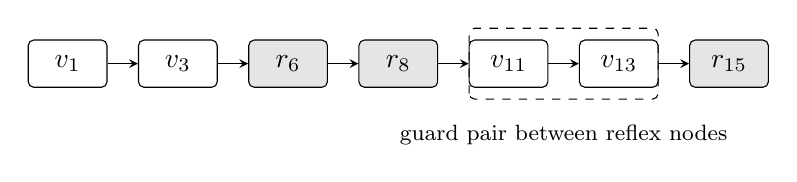
\begin{tikzpicture}[
  node/.style={draw, rounded corners=2pt, minimum width=10mm, minimum height=6mm, inner sep=1pt},
  reflex/.style={node, fill=black!10},
  guard/.style={node, fill=white},
  >=stealth
]
  % Example list from the provided figure: v1 v3 r6 r8 v11 v13 r15
  \node[guard] (v1) at (0,0) {$v_1$};
  \node[guard] (v3) at (1.4,0) {$v_3$};
  \node[reflex] (r6) at (2.8,0) {$r_6$};
  \node[reflex] (r8) at (4.2,0) {$r_8$};
  \node[guard] (v11) at (5.6,0) {$v_{11}$};
  \node[guard] (v13) at (7.0,0) {$v_{13}$};
  \node[reflex] (r15) at (8.4,0) {$r_{15}$};
  \draw[->] (v1) -- (v3);
  \draw[->] (v3) -- (r6);
  \draw[->] (r6) -- (r8);
  \draw[->] (r8) -- (v11);
  \draw[->] (v11) -- (v13);
  \draw[->] (v13) -- (r15);
  \draw[dashed, rounded corners=2pt] (5.1,-0.45) rectangle (7.5,0.45);
  \node at (6.3,-0.9) {\footnotesize guard pair between reflex nodes};
\end{tikzpicture}
\caption{Reflex list \(L(C)\) schematic: reflex extrema (shaded) and guard vertices (white). Between consecutive reflex nodes there may be either 0 guards or exactly 2 guards; the 2-guard block is the \emph{candidate pair} used in merge processing.}
\label{fig:reflex-list-schematic}
\end{figure}

\paragraph{Invariant (no hidden reflex extrema below the current step).}
Let \(r\) be the next reflex extremum of \(C\) processed in increasing \(y\)-order.
Then any boundary arc of \(B(C)\) that lies strictly below height \(y(r)\) contains \emph{no active reflex extrema}.
This is immediate from the processing order if every time we process a reflex extremum \(q\) we cut off (remove) the part of the component strictly below \(y(q)\).
This invariant is the crux behind both correctness (W1) and linear-time walking (W2).

\paragraph{Split step (reflex local maximum).}
Suppose \(r\) is a split vertex in component \(C\).
The report's Case~1 describes finding the chord supports by advancing two boundary iterators outward from a constant-size neighborhood of \(r\) in \(L(C)\) until their incident edges cross the horizontal line \(y=y(r)\).
We can express the operation abstractly:
\begin{itemize}
  \item Choose two guard-adjacent boundary iterators \(L\) (left side) and \(R\) (right side) associated with \(r\)'s neighborhood in \(L(C)\).
  \item Advance \(L\) and \(R\) monotonically along \(B(C)\) until the edges they reference are the first boundary edges hit by the horizontal rays from \(r\) to \(-\infty\) and \(+\infty\) (these are the chord supports).
  \item Insert intersection nodes \(v,w\) on those support edges and splice \(B(C)\) to remove the subpolygon strictly below \(y(r)\) bounded by \(r\) and the two support intersections.
  \item Update \(L(C)\) by removing \(r\) and the guards consumed by the search, and inserting the new guards \(v,w\) tagged with \(\mathrm{below}(v)=\mathrm{below}(w)=r\).
  \item In the chord graph \(G\), connect \(r\) downward to any non-null \(\mathrm{below}(\cdot)\) pointers carried by the consumed guards (this matches the report's ``connect to \(v_k,v_m\) if their pointers are nonzero'').
\end{itemize}

\paragraph{Merge step (reflex local minimum).}
Suppose \(r\) is a merge vertex in component \(C\).
The report's Case~2 can be rephrased using the ``adjacent guard pair'' invariant:
we scan \emph{adjacent guard pairs} \((g_L,g_R)\) in \(L(C)\) (each sitting between consecutive reflex nodes)
until we find one whose lifted support edges at height \(y(r)\) bracket \(r\),
and then we split the component into two along the resulting chord.
For the EQ-weak path, the key requirement is that this scan be implemented as a \emph{walk on the guard pairs} with a linear total bound.
\begin{itemize}
  \item Maintain a current candidate adjacent guard pair \((g_L,g_R)\) on the ``floor'' of \(C\) in \(L(C)\).
  \item Advance \(g_L\) leftward and \(g_R\) rightward along \(B(C)\) until their incident edges cross \(y(r)\).
  \item If the resulting support intersections do not bracket \(r\), move to the neighboring adjacent guard pair in \(L(C)\) and continue.
  \item Once bracketed, insert intersection nodes \(v,w\) and split \(B(C)\) into two components by connecting \(r\) to \(v\) (left component) and to \(w\) (right component), updating the two new reflex lists by placing new guards tagged with \(\mathrm{below}(\cdot)=r\).
\end{itemize}
\emph{Important:} to preserve the \(O(n)\) walking bound, this merge search must be expressible so that each boundary edge is advanced past only \(O(1)\) times globally; otherwise merge handling can become \(\Theta(k_r^2)\) in the worst case.

\paragraph{A concrete merge search (what ``scan non-reflex pairs'' means).}
The phrase ``for each pair of non-reflex vertices \(v_i,v_j\) of the reflex list'' in \texttt{original\_paper.txt} is naturally interpreted as:
\emph{iterate adjacent guard pairs \((g_L,g_R)\) in \(L(C)\)} (i.e., the 2-guard blocks between consecutive reflex nodes),
and for each such pair advance its two boundary iterators until their incident edges cross the horizontal line through \(r\).
Below is a deterministic realization that matches this description.

\begin{algorithm}[H]
\caption{\textsc{MergeSupportsWalk}\((C,r)\): BST-free predecessor by adjacent guard-pair walk}
\label{alg:merge-supports-walk}
\begin{algorithmic}[1]
\Require Component \(C\) with boundary list \(B(C)\) and reflex list \(L(C)\); merge reflex extremum \(r\in C\)
\Ensure Support edges \((e_L(r),e_R(r))\) hit by horizontal rays from \(r\) in \(C\)
\State Let \(y\gets y(r)\), \(x\gets x(r)\)
\State Choose a starting adjacent guard pair \((g_L,g_R)\) in \(L(C)\) \Comment{e.g., a per-component cursor; if none, the nearest 2-guard block around \(r\)}
\While{true}
  \State \(e_L \gets \textsc{LiftLeft}(B(C), g_L, y)\); let \(x_L\) be the \(x\)-coordinate of \(e_L\cap\{Y=y\}\)
  \State \(e_R \gets \textsc{LiftRight}(B(C), g_R, y)\); let \(x_R\) be the \(x\)-coordinate of \(e_R\cap\{Y=y\}\)
  \If{$x_L \le x \le x_R$}
    \State \Return \((e_L,e_R)\)
  \ElsIf{$x < x_L$}
    \State Move to the previous adjacent guard pair in \(L(C)\): \((g_L,g_R)\gets \textsc{PrevGuardPair}(L(C), g_L)\)
  \Else
    \State Move to the next adjacent guard pair in \(L(C)\): \((g_L,g_R)\gets \textsc{NextGuardPair}(L(C), g_R)\)
  \EndIf
\EndWhile
\end{algorithmic}
\end{algorithm}

\paragraph{\textsc{LiftLeft}/\textsc{LiftRight} (the only pointer-walking work).}
Each lift procedure takes a guard node \(g\in L(C)\) and advances a boundary iterator along \(B(C)\) (leftwards for \textsc{LiftLeft}, rightwards for \textsc{LiftRight})
until the incident boundary edge crosses the query height \(y\).
The procedure returns that first crossing edge.
Crucially, since we process reflex extrema in increasing \(y\), each guard can store its current boundary iterator and only move it \emph{forward} as \(y\) increases.

\paragraph{\textsc{NextGuardPair}/\textsc{PrevGuardPair} (pure list navigation).}
Because candidate pairs are exactly the 2-guard blocks between consecutive reflex nodes in \(L(C)\),
the ``next'' candidate pair after a guard \(g_R\) is obtained by walking forward in \(L(C)\) until the next guard node is encountered.
By the invariant, guard nodes appear in consecutive pairs, so the next two guard nodes are \((g'_L,g'_R)\).
The previous candidate pair is symmetric: walk backward from \(g_L\) until the previous guard node is encountered, and take the preceding two-guard block.
These operations are \(O(1)\) amortized per step in the scan (each move skips a run of reflex nodes, and the number of reflex nodes is \(O(k_r)\)).

\paragraph{Key structural claim needed for a clean proof.}
To turn \Cref{alg:merge-supports-walk} into a publishable EQ-weak argument, we want the following monotonicity fact:
\begin{quote}
\textbf{(M) Noncrossing floor intervals:} At height \(y=y(r)\) of the current lowest active merge vertex \(r\) in component \(C\),
each adjacent guard pair \((g_L,g_R)\) defines a unique left/right crossing of \(\{Y=y\}\) on its two incident boundary arcs, producing an \(x\)-interval \([x_L,x_R]\).
Moreover, these intervals are disjoint and appear in the same cyclic order as the corresponding guard pairs in \(L(C)\).
\end{quote}
If (M) holds, then the direction choice in \Cref{alg:merge-supports-walk} cannot ``bounce'': when \(x<x_L\) we must move left in \(L(C)\), and when \(x>x_R\) we must move right.
Thus the scan over guard pairs is a monotone walk, and across the whole algorithm every guard pair is entered only \(O(1)\) times before the component is split or the relevant floor intervals become dead.

\begin{lemma}[Disjointness and order of floor intervals (formalizing (M))]
\label{lem:floor-intervals}
Fix a component \(C\) and a query height \(y\) that is equal to the \(y\)-coordinate of the next (lowest) active merge vertex \(r\) in \(C\).
For every adjacent guard pair \((g_L,g_R)\) in \(L(C)\), let \(A_L(g_L)\) be the boundary arc of \(B(C)\) incident to \(g_L\) on the left side of the floor pocket,
and let \(A_R(g_R)\) be the corresponding arc incident to \(g_R\) on the right side.
Assume general position (no boundary vertex lies exactly on \(\{Y=y\}\)).
Then:
\begin{itemize}
  \item each arc \(A_L(g_L)\) and \(A_R(g_R)\) intersects the line \(\{Y=y\}\) in exactly one point (a unique crossing on an edge),
  \item the resulting intervals \([x_L(g_L),x_R(g_R)]\) are pairwise interior-disjoint,
  \item and their left-to-right order matches the cyclic order of the corresponding guard pairs around \(L(C)\).
\end{itemize}
\end{lemma}

\begin{proof}[Proof sketch]
Each adjacent guard pair corresponds (by invariant) to a processed pocket bounded by two disjoint boundary arcs of \(B(C)\) that are adjacent at the floor.
Since \(r\) is the lowest active merge, there are no active reflex extrema strictly below \(y\), hence no unprocessed ``pockets within pockets'' below \(y\);
in particular, the floor arcs for distinct guard pairs are disjoint subchains of the boundary.
In general position, each such subchain must cross the horizontal line \(\{Y=y\}\) exactly once on each side (otherwise \(\{Y=y\}\) would either miss the pocket completely or intersect it multiple times, contradicting planarity of a simple boundary and the fact that the pocket is already cut off below).
Disjointness and order then follow from planarity: two distinct boundary subchains cannot cross each other, so their intersection \(x\)-coordinates with a fixed horizontal line preserve cyclic order.
\end{proof}

\begin{lemma}[Edge-ownership charging for lifts]
\label{lem:edge-ownership}
Maintain, for each guard node \(g\), a boundary iterator \(\it(g)\) used by \textsc{LiftLeft}/\textsc{LiftRight}, and require that \(\it(g)\) only moves forward along the boundary arc that is incident to \(g\) and belongs to \(g\)'s current floor pocket.
If every boundary edge of every component belongs to at most one such incident arc on each side (left/right) at any time,
then the total number of iterator-advances performed by all lift operations over the whole algorithm is \(O(n)\).
\end{lemma}

\begin{proof}[Proof sketch]
Charge each iterator advance to the boundary edge it steps over.
By the ownership requirement, any active boundary edge can be charged by at most one left-lift iterator and at most one right-lift iterator before it is removed (cut off) or becomes part of a processed floor interval that is never traversed again.
Thus each original boundary edge is charged \(O(1)\) times, implying \(O(n)\) total advancement.
\end{proof}

\paragraph{What the updates must guarantee (split/merge splice rules).}
To actually \emph{use} \Cref{lem:floor-intervals,lem:edge-ownership}, we must specify how \(B(C)\) and \(L(C)\) change after processing a reflex extremum \(r\) so that:
\begin{itemize}
  \item the ``2 guards between consecutive reflex nodes'' invariant remains true, and
  \item edge ownership remains true (edges are not walked by multiple guards).
\end{itemize}
Below is a minimal, implementation-oriented rule set consistent with \texttt{original\_paper.txt}.

\paragraph{Split update (reflex local maximum, Case 1 in \texttt{original\_paper.txt}).}
Let \(r\) be the lowest active split vertex in component \(C\).
Let \(g^-_r\) and \(g^+_r\) be the closest guard nodes to \(r\) in \(L(C)\) on the left and right, respectively (if a side has no guard adjacent to \(r\), treat the closest reflex neighbor as providing a degenerate guard that points to the adjacent boundary vertex in \(B(C)\)).
Run lifts outward from these two guards at height \(y(r)\) to obtain support edges \((e_L(r),e_R(r))\).
Then perform:
\begin{itemize}
  \item \textbf{Cut-off:} remove from the active boundary \(B(C)\) the maximal boundary subchain that lies strictly below \(y(r)\) between the two support edges and is incident to \(r\).
  \item \textbf{Reflex-list rewrite:} remove \(r\) from \(L(C)\); remove any guard nodes whose owned arcs were entirely cut off; insert a new adjacent guard pair \((g_L^{\mathrm{new}},g_R^{\mathrm{new}})\) between the two reflex neighbors of \(r\) in \(L(C)\), and set \(\mathrm{below}(g_L^{\mathrm{new}})=\mathrm{below}(g_R^{\mathrm{new}})=r\).
  \item \textbf{Ownership:} initialize \(\it(g_L^{\mathrm{new}})\) to the boundary position immediately above the left support, and \(\it(g_R^{\mathrm{new}})\) analogously on the right.
  From this point on, \(\it(g_L^{\mathrm{new}})\) (resp.\ \(\it(g_R^{\mathrm{new}})\)) is the unique iterator allowed to traverse boundary edges on that incident side until those edges are cut off by a later step.
\end{itemize}
Intuitively: the new guard pair encodes the new ``floor pocket'' created by processing \(r\), and owns the two incident arcs that future lifts will traverse.

\paragraph{Merge update (reflex local minimum, Case 2).}
Let \(r\) be the lowest active merge vertex in component \(C\).
Run \textsc{MergeSupportsWalk}\((C,r)\) to identify an adjacent guard pair \((g_L,g_R)\) whose lifted crossings at height \(y(r)\) bracket \(r\), yielding \((e_L(r),e_R(r))\).
Then:
\begin{itemize}
  \item \textbf{Split:} split \(C\) into two components \(C_{\text{left}},C_{\text{right}}\) by cutting along the chord supports of \(r\) (conceptually: sever \(B(C)\) at the two support locations and attach each severed side to \(r\) to form two cycles, as described in \texttt{original\_paper.txt}).
  \item \textbf{Reflex-list split:} split \(L(C)\) into two cyclic lists \(L(C_{\text{left}})\) and \(L(C_{\text{right}})\) consistent with the new boundary cycles.
  In each new list, replace the used guard pair by a new adjacent guard pair tagged with \(\mathrm{below}(\cdot)=r\) to represent the new floor pocket created at the split.
  \item \textbf{Ownership:} transfer iterators \(\it(\cdot)\) for all untouched guard pairs to the corresponding new component; initialize iterators for the two new guard pairs adjacent to \(r\) to the boundary positions immediately above the respective supports.
\end{itemize}

\paragraph{Preservation claim (what we need to prove next).}
The remaining (publishability-critical) step is a clean proof that the above split/merge updates preserve:
\begin{itemize}
  \item the structural invariant of \(L(C)\) (0-guards or 2-guards between consecutive reflex nodes),
  \item the disjointness/ordering property of floor intervals (Lemma~\ref{lem:floor-intervals}),
  \item and edge ownership (Lemma~\ref{lem:edge-ownership}).
\end{itemize}
With those in place, (W2) becomes a direct corollary, and (W1) reduces to the ray-shooting lemma under the ``no hidden reflex extrema below'' invariant.

\begin{lemma}[Preservation under split update]
\label{lem:preserve-split}
Assume component \(C\) satisfies the reflex-list invariant and edge-ownership invariant before processing a split vertex \(r\).
After performing the Split update described above (cut off the region strictly below \(y(r)\), remove consumed guards, and insert one new adjacent guard pair tagged by \(r\)),
the resulting component \(C'\) satisfies:
\begin{itemize}
  \item the reflex-list invariant (between consecutive reflex nodes: 0 guards or exactly 2 guards),
  \item the edge-ownership invariant (each active boundary edge is traversable by at most one guard iterator per side),
  \item and the floor-interval disjointness/order property at any later query height \(y'>y(r)\) (Lemma~\ref{lem:floor-intervals} continues to apply).
\end{itemize}
\end{lemma}

\begin{proof}[Proof sketch]
Only the boundary edges in the cut-off subchain are removed; all remaining boundary arcs are unchanged.
In \(L(C)\), the only local modification is replacing a neighborhood containing \(r\) and its consumed guards by a single new 2-guard block \((g_L^{\mathrm{new}},g_R^{\mathrm{new}})\) between \(r\)'s two reflex neighbors.
Thus the ``0-or-2'' structure is preserved everywhere else, and holds at the replacement site by construction.

For ownership: all iterators attached to removed guards disappear together with their owned arcs.
The two new guards are initialized at the two chord supports and are declared the unique owners of the two incident arcs of the new floor pocket; no other guard's owned arc overlaps them because those arcs are newly exposed boundary above the supports.
Hence no surviving boundary edge gains a second owner on either side.

Finally, floor intervals remain disjoint/ordered because the update does not create crossings: it removes a simply connected subpolygon and introduces a new pocket boundary whose two incident arcs are subchains of the original boundary.
Planarity implies the induced intersections with any horizontal line above \(y(r)\) preserve order, so Lemma~\ref{lem:floor-intervals} remains valid for later steps.
\end{proof}

\begin{lemma}[Preservation under merge update]
\label{lem:preserve-merge}
Assume component \(C\) satisfies the reflex-list invariant, the floor-interval property (Lemma~\ref{lem:floor-intervals}) at the merge height \(y(r)\),
and the edge-ownership invariant before processing a merge vertex \(r\).
After performing the Merge update described above (split \(C\) into \(C_{\text{left}},C_{\text{right}}\) along the chord supports, split \(L(C)\), and replace the used guard pair by new guard pairs tagged by \(r\)),
each new component satisfies the reflex-list and edge-ownership invariants, and Lemma~\ref{lem:floor-intervals} applies to future merge processing within each component.
\end{lemma}

\begin{proof}[Proof sketch]
The merge split partitions the boundary cycle into two boundary cycles by cutting at the two support locations and reconnecting through \(r\).
This operation does not introduce self-intersections because the supports are found by horizontal ray shooting and the chords lie inside the polygon.
Thus each resulting cycle is a simple component boundary.

On the reflex list: splitting \(L(C)\) at the used guard pair and distributing nodes according to which boundary cycle they lie on preserves the cyclic order of nodes along each new boundary.
Within each new component, any pre-existing 2-guard blocks remain intact (they lie on one side of the split), and the used block is replaced by one new 2-guard block adjacent to \(r\) by construction.
Hence the 0-or-2 structure holds.

On ownership: every pre-existing guard keeps ownership of exactly the same boundary arc, now residing in exactly one of the two new components.
The only new owners are the two new guard pairs adjacent to \(r\), whose owned arcs are disjoint subchains immediately above the supports on each side.
No surviving guard owned those arcs previously (they were not on any floor pocket boundary), so ownership remains unique.

Finally, floor-interval disjointness/order is preserved within each new component by planarity: the split is along a chord supported by the ray-shooting edges, so it cannot interleave two previously disjoint floor pockets.
Therefore Lemma~\ref{lem:floor-intervals} continues to hold component-wise for subsequent merge steps.
\end{proof}

\paragraph{Corollary (W2 from preservation + ownership).}
Under the update rules and preservation lemmas above, the edge-ownership invariant holds at all times.
Therefore Lemma~\ref{lem:edge-ownership} applies globally, implying the total work of all lift pointer-walks is \(O(n)\).

\paragraph{Why this can be \(O(n)\) total walking (the intended charging argument).}
Assume that every time a boundary iterator advances past an edge \(e\) during some lift,
either (i) \(e\) lies strictly below the chord(s) inserted at that step and is immediately removed from the active component(s), or
(ii) \(e\) becomes part of a processed floor interval delimited by a guard pair and will never again be traversed by any lift.
Then each original boundary edge is charged \(O(1)\) times, giving (W2).
This is exactly the proof idea stated at the end of \texttt{original\_paper.txt}: ``each edge is checked once by the non-reflex pointers.''

\paragraph{Lemma target for (W2).}
\emph{(Charging lemma)} If every advancement of a guard iterator along \(B(C)\) crosses a boundary edge that is removed from further consideration immediately after the current step (either because it lies in the cut-off pocket, or because it becomes part of a processed floor interval), then the total number of iterator advances over the whole run is \(O(n)\).

\paragraph{Lemma target for (W1).}
\emph{(Ray-shooting lemma)} Under the ``no hidden reflex extrema below'' invariant, the first boundary edges hit by horizontal rays from a reflex extremum \(r\) at height \(y(r)\) must lie on the boundary arcs adjacent to \(r\)'s neighborhood in \(L(C)\), so the guard-walk support discovery returns exactly \(\textsc{LeftEdge}(C,r)\) and \(\textsc{RightEdge}(C,r)\).
\medskip

\noindent The remaining work for a publishable EQ-weak proof is to:
\begin{itemize}
  \item state the merge search precisely (as a two-pointer walk on the floor guards), and
  \item prove that both split and merge updates preserve the reflex-list invariant and satisfy the charging lemma.
\end{itemize}

\subsection{Direction B: keep the fixed chain order as a linked list + ``finger'' search}
Since chain order does not swap, we can maintain the active chains as a doubly-linked list in left-to-right order.
To answer ``left of \(v\)'', instead of a BST predecessor query we try to start from a nearby \emph{finger} (previous answer) and walk left/right in the list until the correct chain is found.

\paragraph{Potential amortization hope.}
If successive event vertices have correlated \(x\)-positions, the finger might move only a small total distance.

\paragraph{Risk.}
In the worst case, event vertices can alternate between far-left and far-right \(x\), which can make total walking \(\Theta(k^2)\).
So this needs either:
\begin{itemize}
  \item a stronger structural claim about event locality in polygons, or
  \item multiple fingers / a skip structure (which begins to resemble a BST again).
\end{itemize}

\subsection{Reality check}
Eliminating \emph{all} ordered-search structures for general predecessor queries is suspicious because predecessor search has known lower bounds.
The promising path is therefore Direction~A: restructure the algorithm so we never ask general predecessor queries, and instead recover the needed ``left chain'' information by local pointer walks that can be charged to the boundary.

\section{Is this direction promising? (my take)}
\begin{itemize}
  \item \textbf{Pros}: potentially much simpler story (``sort reflex extrema, walk pointers, emit diagonals''), and naturally highlights instance sensitivity.
  \item \textbf{Cons}: making it both (i) \emph{fully correct} and (ii) \emph{actually simpler than a chain-based sweep} is non-trivial; the chord construction risks re-deriving the classical sweep implicitly.
\end{itemize}

\paragraph{Recommendation.}
Promising as a \emph{presentation} direction (a simpler narrative for essentially the same mechanism).
As a \emph{new algorithm}, we should be cautious: to be publishable, we likely still need an equivalence-to-sweep proof or a clean monotone-invariant argument.

\end{document}

